
\begin{frame}[t,allowframebreaks]{
    Learning rate decay -}

    The \index{learning rate}\gls{learning rate}
    is {\em `the single most important 
    \index{hyperparameter}\gls{hyperparameter}'} \cite{Bengio:2012gbt}.\\
    \vspace{0.1cm}

    Using a constant \gls{learning rate} is often very inefficient.\\

    \begin{columns}
        \begin{column}{0.55\textwidth}
            \begin{center}
                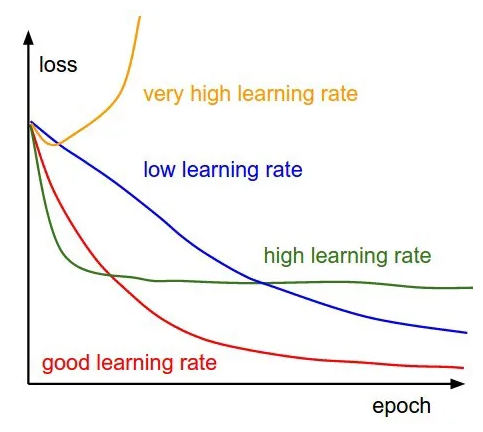
\includegraphics[width=0.98\textwidth]
                    {./images/training_issues/lathiya20_loss_function_various_learn_rates.png}\\
                {\tiny 
                    \color{col:attribution} 
                    Schematic taken from \cite{Medium:LRateDecay}.\\
                }
            \end{center}                
        \end{column}
        \begin{column}{0.45\textwidth}
            \begin{itemize}
                \small
                \item
                With a lower rate, the algorithm may take 
                too long to reach an optimal solution, 
                and it may be easily stuck in a local minimum.\\
                \vspace{0.2cm}
                \item 
                With a higher rate, the algorithm can bounce around 
                the optimal position and fail to converge.\\
            \end{itemize}        
        \end{column}
    \end{columns}

    \framebreak

    %
    %

    \begin{center}

        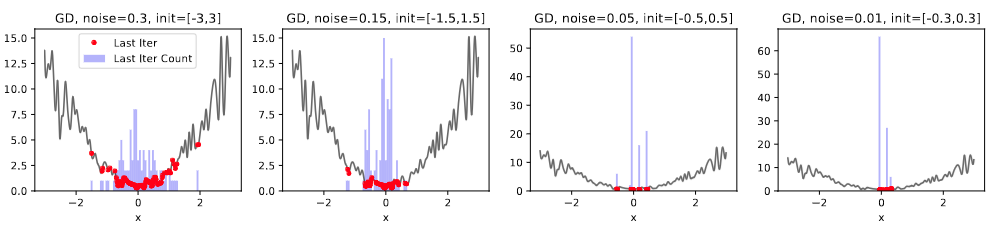
\includegraphics[width=0.93\textwidth]
            {./images/training_issues/kleinberg18_loc_min_various_learn_rates.png}\\
        {\scriptsize
        An initial large learning rate helps escape local minima.
        Subsequent rounds of rate decay (plots 2-4 from the left) increase the 
        likelihood of reaching the true minimum.
        \color{col:attribution} 
            \tiny Plot taken from \cite{Kleinberg:2018gdlm}.\\
        }

        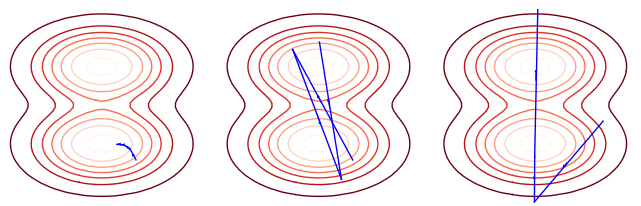
\includegraphics[width=0.87\textwidth]
            {./images/training_issues/you19_3_learning_rates.png}\\
        {\scriptsize
        From left to right: 
        1) learning rate is small enough to converge around a minimum, 
        2) moderate so that it bounces among minima, 
        3) too large to converge.
        \color{col:attribution} 
            \tiny Schematic taken from \cite{You:2019lrd}.\\
        }
    \end{center}        

    \framebreak

    %
    %

    Ideally, we want to take:
    \begin{itemize}
        \item
        larger steps when we are still away from the optimal solution, and
        \item
        smaller steps when we are close to it.
    \end{itemize}

    \vspace{0.1cm}

    A \index{learning rate}\index{learning rate decay} 
    \gls{learning rate decay} {\bf can achieve the desired adjustment}.

    \vspace{0.2cm}

    Decay is {\bf empirically proven} to improve the learning process.

    \vspace{0.2cm}

    Typically, the following {\em exponential} and {\em inverse} decay functions
    are most commonly used to set the \gls{learning rate} $\alpha_n$
    used at the training \index{epoch}\gls{epoch} $n$:\\
    \begin{equation}
        \alpha_n = \alpha_0 e^{-kn}
    \end{equation}
    \begin{equation}
        \alpha_n = \frac{\alpha_0}{1+kn}
    \end{equation}
    where $k$ controls the rate of decay and $\alpha_0$ is the initial rate.

    \vspace{0.2cm}

    Another approach is to reduce $\alpha$ by a fixed factor every few \glspl{epoch}.

\end{frame}
